\documentclass[12pt,a4paper,twoside,titlepage]{memoir}
\usepackage[utf8]{inputenc}
\usepackage{amsmath}
\usepackage{amsfonts}
\usepackage{amssymb}
\usepackage{graphicx}
\usepackage{color}
\usepackage{tabularx}
\newcommand{\todo}{\textcolor{red}{\textbf{TODO}}}
\newcommand{\UB}{\textit{upper body}}
\newcommand{\LB}{\textit{lower body}}
\newcommand{\FB}{\textit{full body}}
\title{Influence of Egocentric and Exocentric Perspectives on Virtual Avatars during Full-Body and Part-Body Mirrored and Independent Motor Learning Tasks}
\date{\today}
\author{Stefan Paul Feyer\\ HCI Group, University of Konstanz}
\begin{document}
	\maketitle
	%\section*{Abstract}
\chapter*{Abstract}

	sfgsdfgsdgsdfgsdfgdsfgdsfgsdfg
\begin{itemize}
	\item Overall aim of the Seminar thesis: how to investigate the influence of perspectives on virtual avatars in MR for motor learning
	\item therefore analysis of motor learning, related work, research questions
	\item propose study setting
\end{itemize}

	\chapter{Introduction}

\section{Motivation}
%heranführung zum thema, erklären warum das wichtig ist.
In recent years, Mixed Reality (MR) devices became affordable \footnote{\hyperlink{https://www.vive.com/}{vive.com}, \hyperlink{https://www.oculus.com/}{oculus.com}accessed: 3.12.2019}, portable \footnote{\hyperlink{https://arvr.google.com/daydream/}{arvr.google.com/daydream} accessed: 3.12.2019} and usable in many conditions. Not only academic researchers are interested in this technology, commercial companies also found MR devices helpful to explore new possibilities to use it profitable. With this development, learning and training in MR became possible for many cases, too. EON \footnote{\hyperlink{https://www.eonreality.com/}{https://www.eonreality.com/} accessed: 14.12.2018} for example calls themself "the world leader in Virtual Reality based knowledge transfer for industry, education, and edutainment". They develop MR programs for several platforms, eg. with the aim to guide workers, reducing mistakes and thus reducing costs. These programs address a lot of use cases in the field of education, energy, health \& medical, manufacturing \& industrial, defence \& security and aerospace. Tasks include eg. ground crew training for a Boeing 777, augmented reality (AR) assembly training, exploring or anatomy simulation to mention only a few, compare \ref{fig:eonreality}.
\begin{figure}
	\centering
	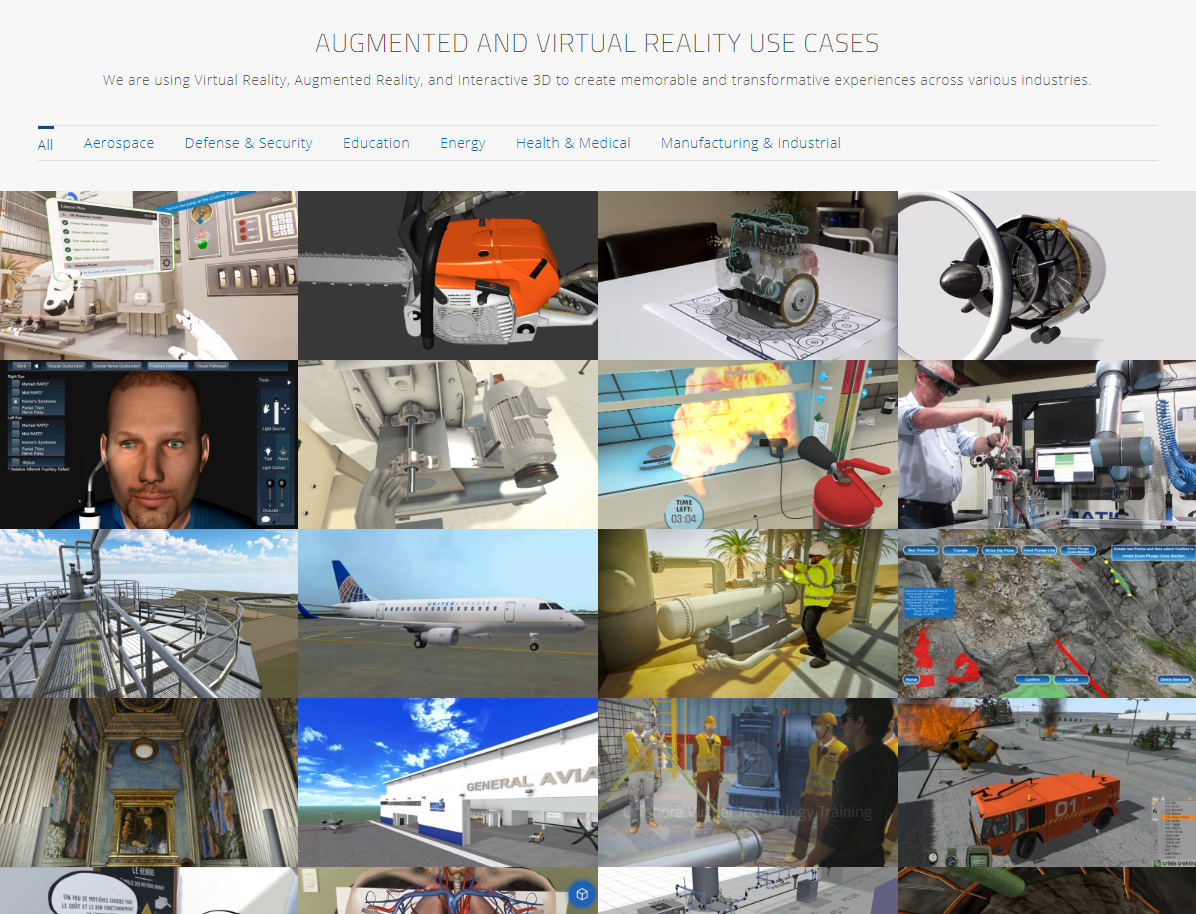
\includegraphics[width=1.0\textwidth]{img/eonreality.PNG}
	\caption{Usecases by EONReality on their AVR plattform.  \hyperlink{https://www.eonreality.com/use-cases/}{eonreality.com/use-cases/} accessed 30.07.2019}
	\label{fig:eonreality}
\end{figure}
Microsoft also stepps into this topic with partners, developing tools for apprentice, maintenance, or remote training. Eg. The Smart Glass experience Lab\footnote{\hyperlink{https://www.fit.fraunhofer.de/de/fb/cscw/smart-glasses-experience-lab.html}{fit.fraunhofer.de/de/fb/cscw/smart-glasses-experience-lab.html} accessed: 18.11.2019} of the Fraunhofer Institute use the MS Hololens \footnote{\hyperlink{https://www.microsoft.com/en-us/hololens}{microsoft.com/en-us/hololens} accessed: 3.12.2019} for remote maintenance, compare figure \ref{fig:fraunhofer}.
\begin{figure}
	\centering
	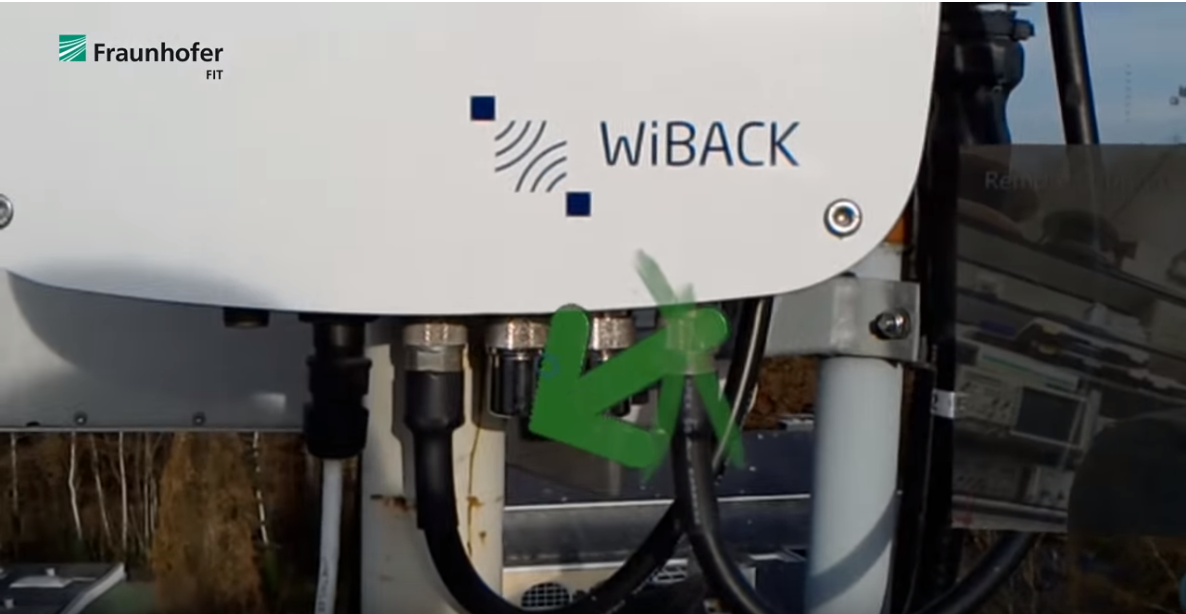
\includegraphics[width=1.0\textwidth]{img/fraunhofer.PNG}
	\caption{Remote maintenance with Hololens by Smart Glass Experience Lab. The on site worker wears a Hololens, while the remote trainer draws green hints to resolve a miswiring, taken from \hyperlink{https://www.youtube.com/watch?v=1QFMPo5k6p0}{https://www.youtube.com/watch?v=1QFMPo5k6p0}, accessed (30.07.2019)}
	\label{fig:fraunhofer}
\end{figure}\\
For developing MR learning and training environments, research put effort in developing how-to's and guidelines to ensure proper systems e.g. \cite{LaViola2017}. However - as we will see in Chapter 3 - there is a research gap about the visual perspective in these systems. For example, a student wants to learn a movement from a teacher. In the real world, the teacher stands in front of the student preforming the movement and the student tries to mimic it. This perspective is called exocentric or 3rd person. In contrast, in MR we have the possibility to change this perspective what we cannot do in the real world. A student can "step into" the teachers virtual body and see the instruction from the 1st person view of the teacher, also called egocentric view. Changing the perspective could have influence on the learning. This rises the following question: Does the perspective has influence on learning in MR environments? 
This seminar thesis is the first out of three parts, followed by a Masters Project and a Masters thesis. The overall aim of this work is to answer the following main research question:
\begin{itemize}
	\item[MRQ] Does the visual perspective on a virtual guidance visualisation have an influence on motor learning in MR environments.
	
\end{itemize}
The outcome in this work is a study design that will be able to address the research questions. In the Masters project the proposed study setting will be implemented, to be able to conduct the study and collecting the necessary data to answer the question. The Masters thesis itself will take the generated data to answer the research question.


\section{Outline}
For a proper study design many aspects must be taken into consideration. The main aspects this thesis will discuss are defined in the following, while further aspects like algorithms are discussed in the masters project. In Chapter 2 this work sets the scope and provides theoretical foundations. in Chapter 3 the parameters for the study design are discussed by means of related work. With the scope and parameters set, Chapter 4 proposes a study design which serves as base for the Masters project. In the end, an outlook on further work on the Masters thesis is given. Compare figure \ref{fig:overallProcess}.
\begin{figure}
	\centering
	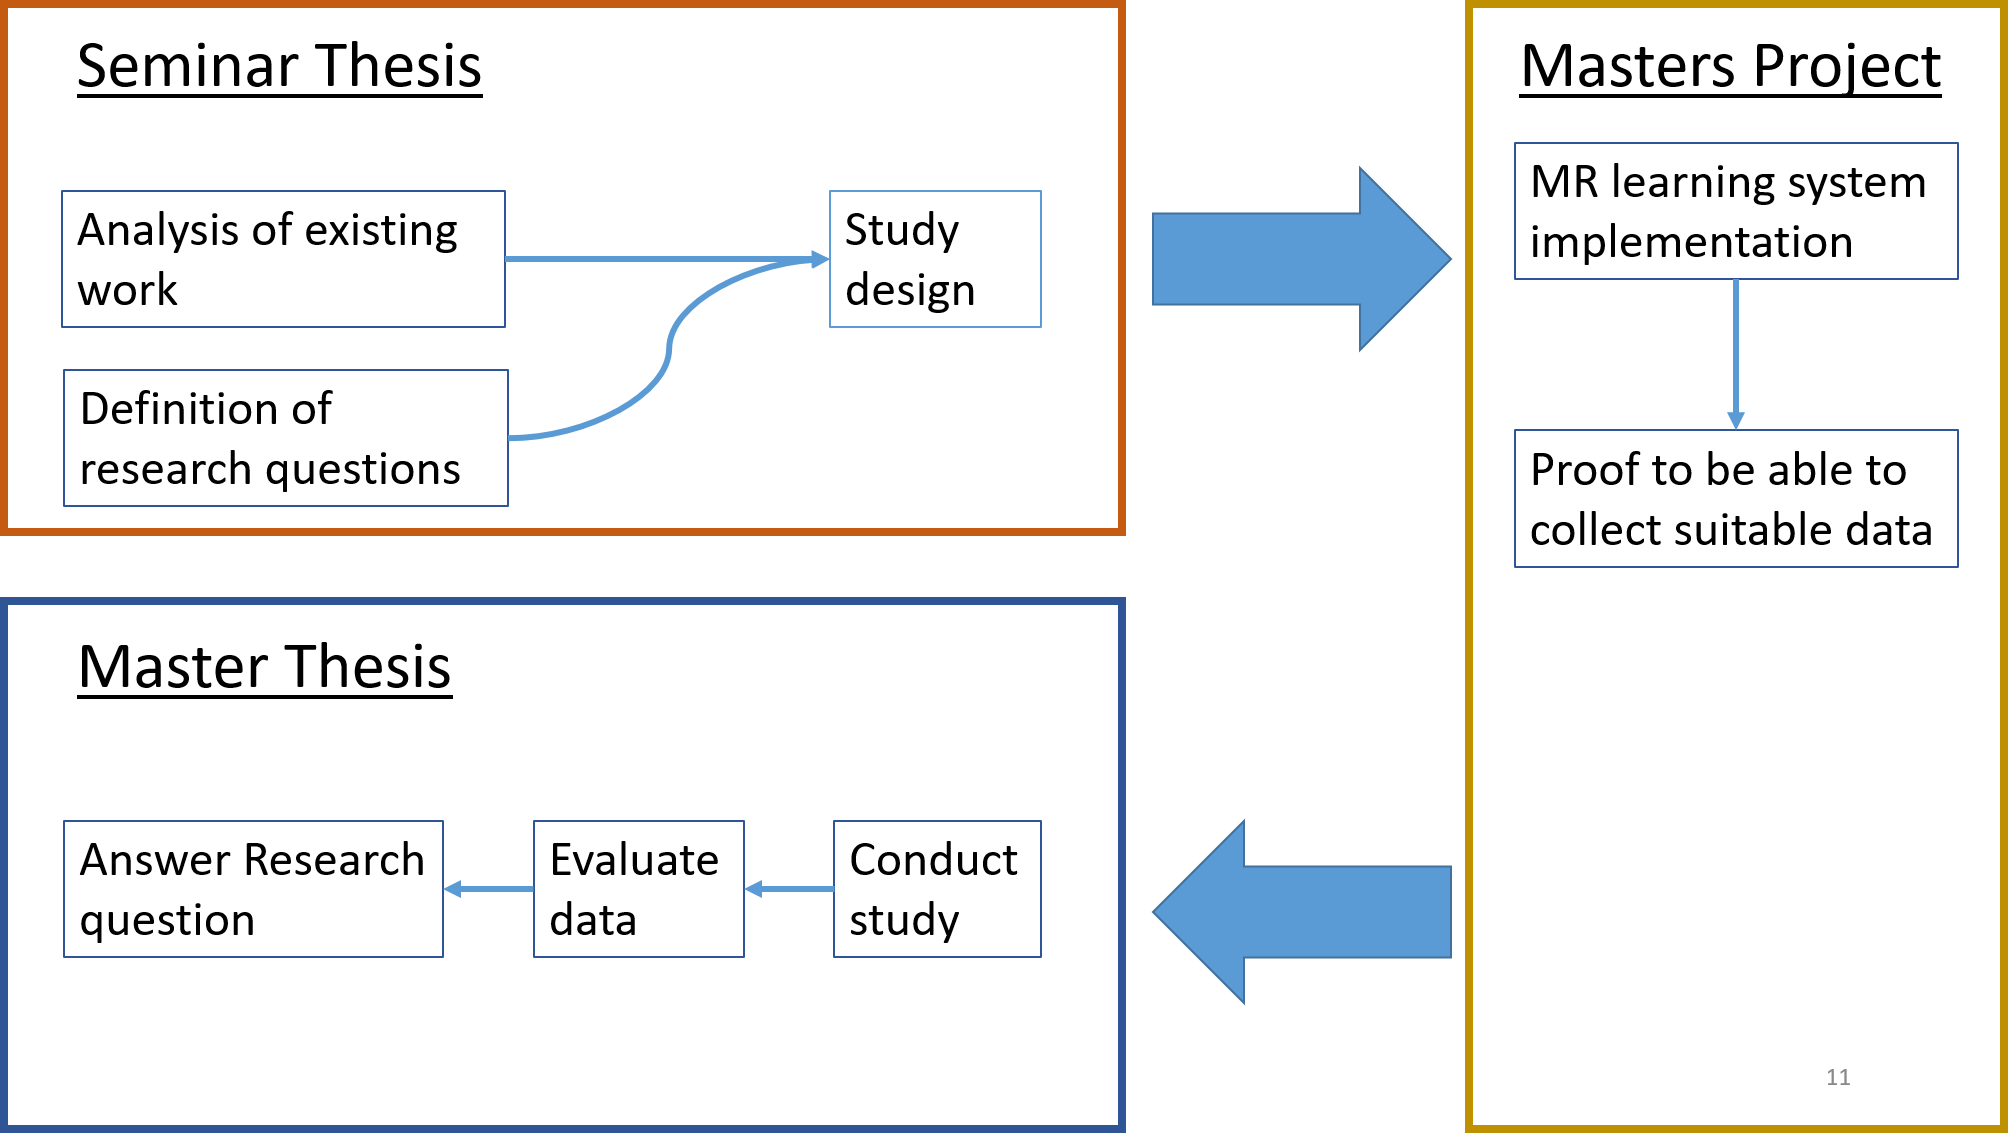
\includegraphics[width=1.0\textwidth]{img/overallProcess.png}
	\caption{Overall process of the masters thesis.}
	\label{fig:overallProcess}
\end{figure}\\

%Each of these aspects must be chosen wisely. In order to do so this seminar thesis will systematically go through every one of them. Chapter 3 sets the scope of the study and provides general knowledge about the domain. The following chapter 4 analyses the work of researchers and their systems, to find suitable components for the scope that has been set in chapter 4. Here, the remaining aspects are analysed from a more practical view and it is investigated how researchers decided about the aspects and why. Whenever a decision is made to be used in the proposed study design, a symbol on the side of the text can be found \markA. After all aspects are clear and reasoned, a study design is proposed in chapter 5. 

%first the theoretical background will be taken into consideration. It is mandatory to know how humans learn, classify, quantify and measure movements. In addition, recent MR hardware and tracking technology is investigated, a classification of perspectives is given and also a insight on MR itself. In this chapter we also set the res
%This seminar thesis will have a look at the grounding principles to define a system that lead to the guidelines in question. Therefore we first step into the theoretical background in the next chapter. We will investigate how people achieve motor skills, how to quantify and measure movements, what hardware techniques are suitable, perspectives and mixed reality. In the following chapter we analyse how other researchers used the theory to gain insights in Motor learing in VR. In the end we propose a study setting to that can be used to investigate on this topic.
%After this introduction, the scope of this thesis is given, where it is explained to what extend motor learning, MR, perspectives and other factors are considered. The following related work part will give an overview about other MR learning systems and also work about perspectives on avatars. From this work the measures, dependent and independent variables and tasks are derived. Taking the related work into consideration a study design is proposed in outlook section.
	\chapter{Scope}
\section{Motor Learning}
%beschreibung welche auf welche art von bewegungen sich hier beschränkt wird.
\begin{itemize}
	\item discrete movements
	\item closed skills
	\item at least 2 different movement categories
	\item how to measure movements
	\item posture vs movement
\end{itemize}

\section{Mixed Reality}
%begründen welchen auf welchen part des kontinuums man sich beschränkt
\begin{itemize}
	\item Milgram
	\item AR or VR
\end{itemize}

\section{Perspective}
%welche prespectiven behandelt werden und welche nicht


\section{Misc}
%welche einschränkungen gibt es noch. zb. das es kein feedback gibt, der realitätsgrad der avatare nicht evaluiert werden soll. erst zum schluss
\begin{itemize}
	\item synchron asynchron
	\item colocated/remote
	\item perspective
	\item hardware?
	\item feedback!
	\item real world, not abstract avatars
	\item only visuals - no audio or textual explanation
\end{itemize}
	\chapter{Theory}
\section{Metholodgy}
sth like UX live cycle or participatory design
\section{HCI Theory}
sth like embodied cognition
Groundwork for designing VR motor learning systems

	\chapter{Related Work}
wie haben die anderen diese variablen untersucht
wie wurden die variablen untersucht $\rightarrow$ studiensetting
%----------------------------------------------------
\section{MR learning systems}


%----------------------------------------------------
\section{Ego/exo perspective work - if exists}

%----------------------------------------------------
\section{variables}
\begin{itemize}
	\item independent/dependent variables
	\item measures
	\item task: reuse or adapt existing task
\end{itemize}
%----------------------------------------------------
\subsection{Task}
\begin{itemize}
	\item Onebody: artificial postures not from but like: tai chi, matial arts
	\item VR Dance Trainer: dance movements
\end{itemize}
%----------------------------------------------------
\subsection{Measures}
\begin{itemize}
	\item onebody
	\item VR Dance trainer
\end{itemize}
%----------------------------------------------------
\section{Body parts included}
\begin{itemize}
	\item onebody
	\item vr dance trainer
	\item 
\end{itemize}
%----------------------------------------------------
\subsection{Independent and Dependent Variables}
\subsubsection{Dependent Variables}
\begin{itemize}
	\item VR
	\item bilateral movements
	\item Movement types: synchronous  / asynchronous 
\end{itemize}
\subsubsection{Independent Variables}
\begin{itemize}
	\item Body parts: upper body (UB), lower body (LB), full body (FB)
	\item Perspective: Ego, Exo, Ego/Exo combined
	\item Movement types: synchronous  / asynchronous 
\end{itemize}

write sth...

%----------------------------------------------------
\section{Conclusion}
\begin{itemize}
	\item task is xyz because of abc
	\item measures are xyz because of abc
	\item variables are...
\end{itemize}

	\chapter{Proposed Study Design}
Given the scope from chapter 2 and the parameters from chapter 3, this chapter proposes a study design. The study aims to produce data to answer the main research question from chapter 1:
\begin{itemize}
	\item[MRQ] Does the visual perspective on a virtual guidance visualisation have an influence on motor learning in MR environments.
\end{itemize}

\section{Setup}
For the study, a movement training system will be implemented. This movement training system will include a virtual reality HMD and motion-tracking technology. The student will be tracked with this motion capturing technology and with the resulting information, the student's avatar will be rendered as a high realism degree avatar. Likewise, the teacher avatar will be rendered, but not on the base of live motion tracking data. A professional Tai Chi trainer will be invited and a Tai Chi form will be recorded. This form will be split into 4 sub-forms. Furthermore, the teacher avatar will be scaled to the size of the student's avatar. To overcome the mirror issue, the student is allowed to move freely around the teachers' avatar. During the students' performance, the movement will be recorded and analysed in the aftermath with the discussed performance measure. 

\section{Procedure}
The study is conducted in a within-subject design with counterbalancing, which results in 32 participants, compare table~\ref{tbl:studySetting}. The student starts with the first visual perspective. The teacher appears and performs the movement, while the student is watching the performance. After the first demonstration, the student can train the motion simultaneously until the student is feeling confident, but caps after an amount of time which a pilot study has to reveal. After one of these cases, the final movement will be recorded, the student gets a short recovery rest. Then the next visual perspective starts. This process continues throughout all four conditions. Subsequent to the actual study, the post questionnaires will be answered. This questionnaire will contain questions about, perceived precision, ease to understand an preferred method.

\begin{table}
	\centering
	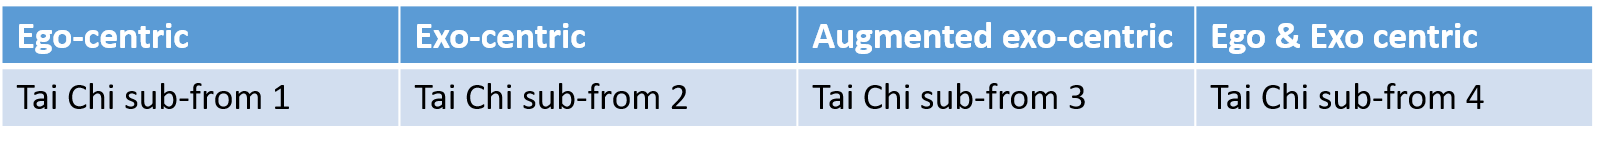
\includegraphics[width=1.0\textwidth]{img/studySetting.png}
	\caption{Study conduction schema.}
	\label{tbl:studySetting}
\end{table}

\section{Outlook}
The next step is to implement the study setup, but still, there are some parameters to refine on. This takes place in the master's project. In this part, the technology and algorithms will be in the main focus. For technology, VR HMDs will be compared and a decision will be made. Similar to motion tracking technologies. After this, algorithms for comparing two movements will be evaluated. When decisions are made, the implementation of the system will start. Eventually, a pilot testing session will take place followed by further refinements.
The milestones for the master's project are:
\begin{itemize}
	\item Hardware requirements: 17.1.2020
	\item Software Requirements: 24.1.2020
	\item Implementation Start: 27.1.2020
	\item Pilot Study: 2.3.2020
	\item Refinements Implementation: 13.3.2020
	\item Master’s Project Presentation and Report: 23.3.2020
\end{itemize}
The thesis will follow in the summer semester 2020. The results are planned to be published at a conference in 2020, compare figure~\ref{fig:outlook}.\\
For the master's thesis, a study will be conducted. The study will generate data to answer the research question. This data will be analysed in detail and eventually be used to answer the research question.

\begin{figure}
	\centering
	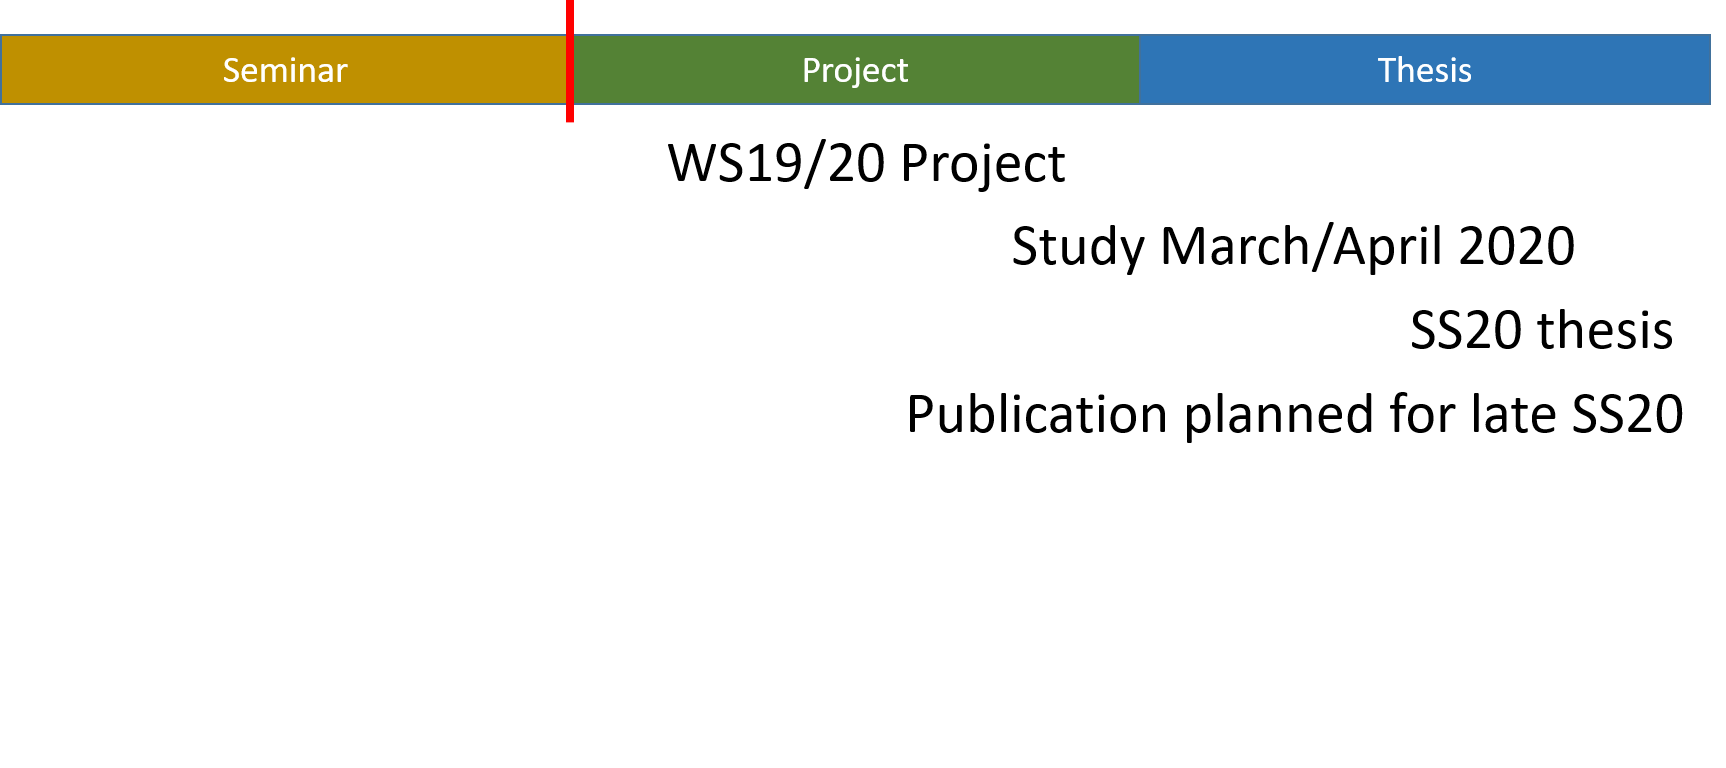
\includegraphics[width=1.0\textwidth]{img/outlook.png}
	\caption{Timetable for the master's thesis.}
	\label{fig:outlook}
\end{figure}

\begin{comment}
\section{Variables}
\subsection{Independent Variables}
\begin{itemize}
\item ego-centric
\item exo-centric
\item combined
\begin{itemize}
\item \textcolor{red}{variation of combined:} sequetial - parallel
\end{itemize}
\end{itemize}
further variations that could be interesting:
\begin{itemize}
\item body parts
\item sitting/standing
\item visual representation
\item degree of realism of avatar
\item guidance techniques: stopping at keyframes vs. fluent instructions
\item audio queues
\item feedback
\item fixed position of teacher and avatar, vs walking around
\end{itemize}
\subsection{Dependent variables}
Score. Combination of objective and subjective measurements.
\begin{itemize}
\item precision
\item subjective opinion of participant
\item stress level (EKG, HRV)
\item cognitive load
\item retention
\item reaction time
\end{itemize}
\section{Task}
\begin{itemize}
\item Tai Chi form, split in subtasks
\item Dance moves from single dance
\end{itemize}
variations:
\begin{itemize}
\item difficulty
\item complexity
\item abstract vs. real world
\item operate a control panel
\item escape the room
\item game    
\end{itemize}

\section{Hypothesis}
%hier wird ein mögliches studiendesign vorgestellt

\subsection{Aim of the Study}
The aim of the study is to investigate the influence of egocentric and exocentric perspectives on a virtual avatar during motor learning tasks.

\subsection{process}
There are two groups: one learn only with the egocentric perspective, the other one with the exocentric perspective on the virtual avatar.\\
To derive conclusions on body regions, every participant learns movements for three different body parts. The body parts are:
\begin{itemize}
\item \UB (UB)
\item \LB (LB)
\item \FB (FB)
\end{itemize}
To derive conclusion on movement types, two different movements per body part is learned. The two movement types are:
\begin{itemize}
\item mirrored movements
\item independent movements
\end{itemize}

\begin{center}
\begin{tabular}{ | c | c | c | c | }
\hline
& UB & LB & FB \\ \hline 
Ego & \parbox{4cm}{1 mirrored and 1 asynchronous movement} & \parbox{4cm}{1 mirrored and 1 independent movement} & \parbox{4cm}{1 mirrored and 1 independent movement} \\ \hline 
Exo & \parbox{4cm}{1 mirrored and 1 independent movement} & \parbox{4cm}{1 mirrored and 1 independent movement} & \parbox{4cm}{1 mirrored and 1 independent movement} \\ \hline
Ego/Exo & \parbox{4cm}{1 mirrored and 1 independent movement} & \parbox{4cm}{1 mirrored and 1 independent movement} & \parbox{4cm}{1 mirrored and 1 independent movement} \\
\hline
\end{tabular}
\label{table:studyDesign}
\end{center}

\subsection{Independent variables}
\begin{itemize}
\item perspective on the avatar (Ego/Exo centric)
\item body parts (\UB, \LB, \FB)
\item movement types (mirrored/independent movements)
\end{itemize}

\subsection{measures}
TBA
\end{comment}
	\chapter{Outlook}
\begin{itemize}
	\item timetable, what to do
\end{itemize}
	%\section{Motivation}
äöü
	%\section{them. verw. arbeiten}
requirements: variablen zu untersuchen
	%\section{conclusion}
	%\section{Motor Learning}
\begin{itemize}
	\item for simplifying discussion introducing classification of movements and motor tasks.
	\item 2 important classification schemes:
	\begin{itemize}
		\item based on particular movements made: discrete, continuous, serial
		\item based on perceptual attributes of the task: open/closed
	\end{itemize}
	\item \underline{discrete movements}
\end{itemize}

	%\section{Zusammenfassungen von gelesenen papern}
\end{document}